\actTitle{1.7 - Piecewise Define Functions and Analysis of Graphs}

\videoLink{Section 1.7}{https://www.youtube.com/playlist?list=PLYHZK3b8UFw0MGYUVN9Z4aYof_QgbFw7f}

\noindent \textbf{Topics:}  basic functions, even and odd functions, graphing piecewise functions, relative minima and maxima\\

\noindent \textbf{Student Learning Outcomes:}
\begin{enumerate}
\item Students will be able to determine whether a function is even, odd, or neither.
\item Students will be able to graph a piecewise function.
\item Students will be able to determine where a function is increasing, decreasing, or constant.
\item  Students will be able to locate relative minimum and relative maximum values of a function on a graph.
\end{enumerate}

\hrule 

\bigskip

\subsection{Even and Odd Functions} ~


\noindent \begin{tabular}{| l |} \hline
We call $f$ an \emph{even} function if the graph of $f$ is symmetric with respect to the $y$ axis.\\ In that case, $f(-x)=f(x)$ for every $x$ in the domain. \\ \hline
\end{tabular}



\noindent \begin{tabular}{| l |} \hline
We call $f$ an \emph{odd} function if the graph of $f$ is symmetric with respect to the origin.\\ In that case, $f(-x)=-f(x)$ for every $x$ in the domain. \\ \hline
\end{tabular}



\begin{enumerate}
\item Determine whether $f$ is even, odd, or neither. 
\begin{enumerate}
\item $f(x)=17x^3-12x^5$\\[1in]
\item $f(x)=x^3-5x^2$\\[1in]
\item $f(x)=|x|$ This is the \emph{absolute value function}. \\[1in]%Sketch its graph below.
\end{enumerate}



\newpage


\subsection{Piecewise-Defined Functions} ~

\hspace{-.4in} \begin{tabular}{| l |} \hline \underline{Piecewise-Defined Functions.}  \\
A \emph{piecewise function} is a function defined by multiple sub-functions with each sub-function applying\\ to a certain interval of the main function's domain.\\
 \hline
\end{tabular}



\item Evaluate the function for the given values of $x$ and then graph the function.
\[
  f(x) =
  \begin{cases}
                                   -x-1 & \text{for $x<1$} \\
                                   -3 & \text{for $1 \leq x <2$} \\
  \sqrt{x-2} & \text{for $x \geq 2$}
  \end{cases}
\]

\begin{enumerate}
\item $f(-3)=$\\[.2in]
\item $f(1)=$ \\[.2in]
\item $f(2)=$ \\[.2in]
\item $f(6)=$ \\[.2in]
\item Graph $f(x)$
\end{enumerate}


\scalebox{0.4}{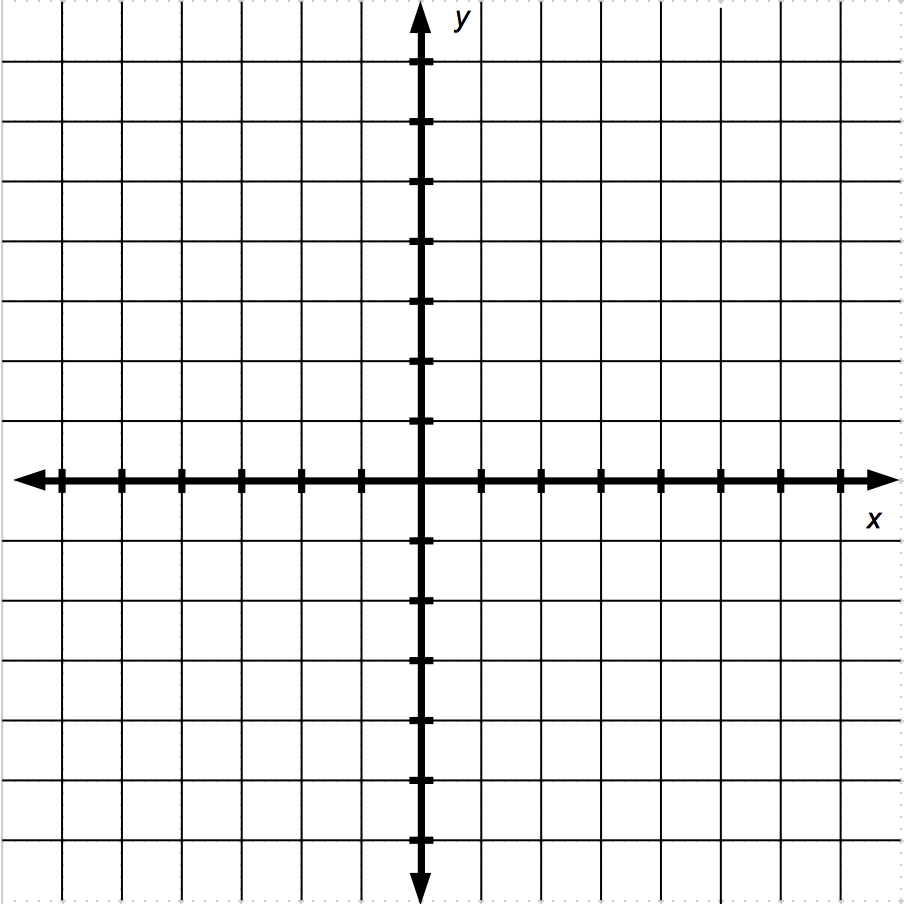
\includegraphics{bigaxes}} 


\newpage



\item Graph the piecewise function.
\[
  f(x) =
  \begin{cases}
                                   x+3 & \text{for $x<-1$} \\
                                   x^2 & \text{for $-1 \leq x <2$} 
  \end{cases}
\]

\scalebox{0.4}{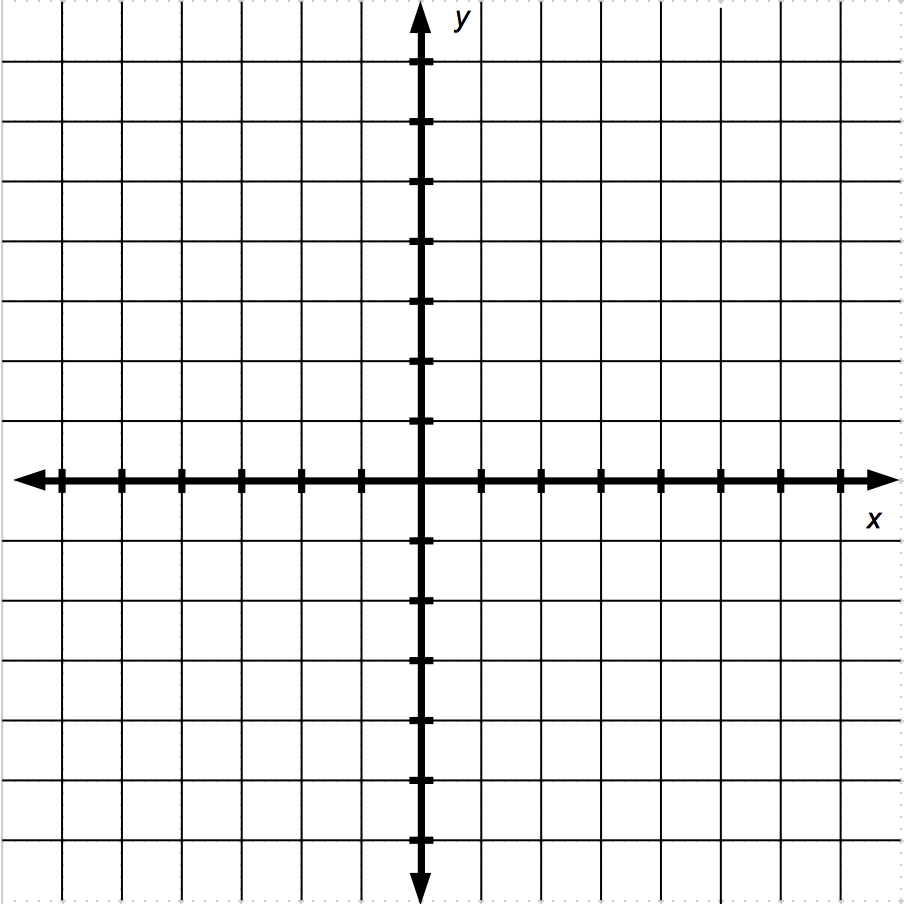
\includegraphics{bigaxes}} 

\subsection{Intervals of Increasing, Decreasing, and Constant Behavior}
When looking at functions on a graph, we read from left to right.
And when we talk about function values, we mean values on the $y$-axis.\\[.1in]

In this section, we will determine intervals on the $x$-axis where the
function values on the $y$-axis are increasing, decreasing, or
constant.

\item Determine where the following function is increasing, decreasing, or constant.\\
\scalebox{0.5}{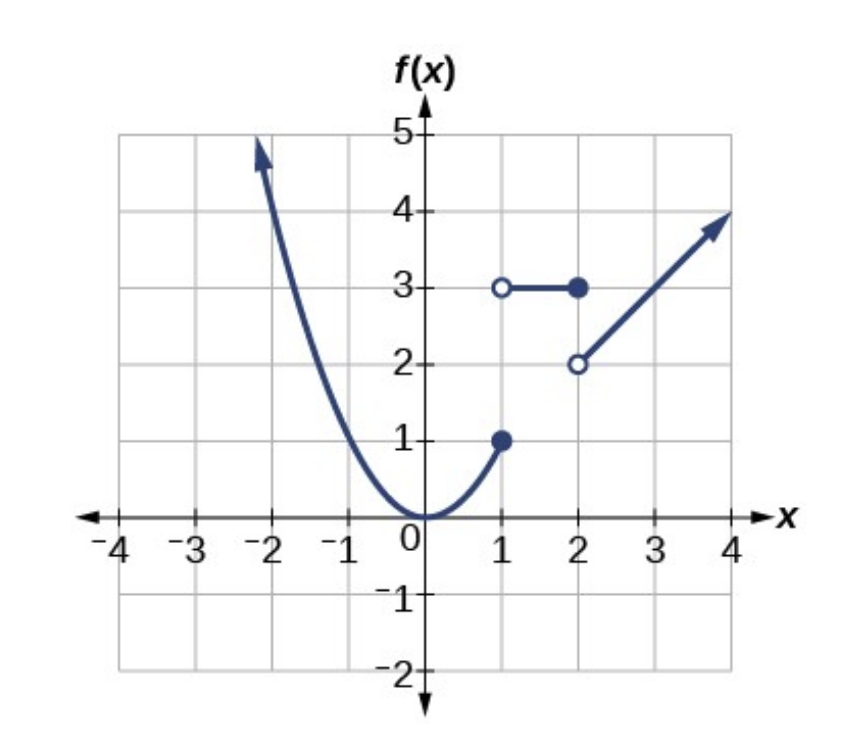
\includegraphics{incrdecr}} 

\newpage

\subsection{Relative Minimum and Relative Maximum Values}
Remember, when talking about function \textbf{values}, we mean
$y$-values.  So in this section we will determine the relative minimum
and maximum $y$-values of a function.

\item For the graph of $y=f(x)$ shown.\\
\scalebox{0.8}{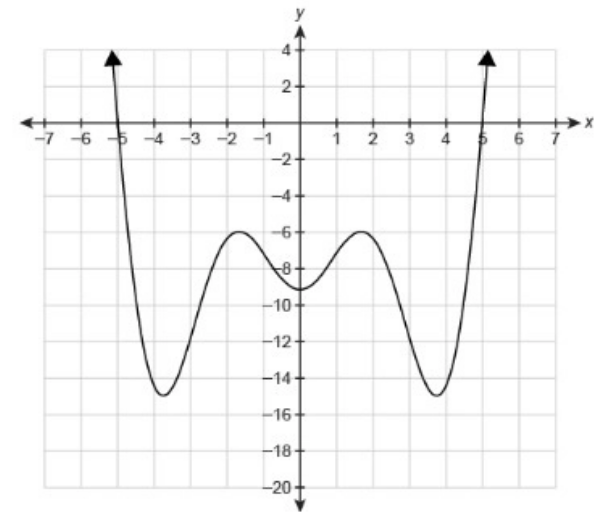
\includegraphics{relminmax}}
\begin{enumerate}
\item Determine the location and value of any relative maxima.\\[.3in]
\item Determine the location and value of any relative minima.
\end{enumerate}

\vfill
\end{enumerate}

\noindent \textbf{Student Learning Outcomes Check}

\begin{enumerate}
\item Can you determine whether a function is even, odd, or neither?
\item Can you graph a piecewise function?
\item Are you able to determine where a function is increasing, decreasing, or constant?
\item  Can you locate relative minimum and relative maximum values of a function on a graph?

\end{enumerate}

\noindent \textbf{If any of your answers were no, please ask about these topics in class.}


